% =====================================================================
%  Parameter Identification for the ZrMicro Irradiation-Microstructure Model
%  DisloCluster — Docs/Formulation/Parameter_Identification.tex
%
%  Compile with:  pdflatex Parameter_Identification.tex   (run twice for refs)
%  Requires a TeX distribution with TikZ and the algorithm/algpseudocode packages.
% =====================================================================
\documentclass[11pt]{article}

\usepackage[a4paper,margin=1in]{geometry}
\usepackage{amsmath,amssymb,amsfonts,bm}
\usepackage{graphicx}
\usepackage{booktabs}
\usepackage{siunitx}
\usepackage{xcolor}
\usepackage{algorithm}
\usepackage{algpseudocode}
\usepackage[numbers,sort&compress]{natbib}
\usepackage[hidelinks]{hyperref}

\usepackage{tikz}
\usetikzlibrary{positioning,arrows.meta,shapes.geometric,calc,fit,backgrounds,decorations.pathreplacing}

% ── TikZ styles for the block diagrams ───────────────────────────────
\tikzset{
  block/.style   = {rectangle, rounded corners, draw=black!70, very thick,
                    fill=blue!6, text width=30mm, minimum height=11mm,
                    align=center, font=\small},
  data/.style    = {rectangle, draw=black!70, very thick, fill=green!8,
                    text width=27mm, minimum height=10mm, align=center, font=\small},
  decision/.style= {diamond, aspect=2, draw=black!70, very thick, fill=orange!12,
                    align=center, font=\small, inner sep=1pt},
  io/.style      = {trapezium, trapezium left angle=70, trapezium right angle=110,
                    draw=black!70, very thick, fill=gray!10, align=center, font=\small,
                    text width=24mm, minimum height=9mm},
  arr/.style     = {-{Stealth[length=2.4mm]}, very thick},
  fbk/.style     = {-{Stealth[length=2.4mm]}, very thick, dashed, red!60!black},
}

\newcommand{\R}{\mathbb{R}}
\newcommand{\param}{\bm{\theta}}
\newcommand{\xv}{\bm{x}}
\newcommand{\NL}{N_{\mathrm{L}}}
\newcommand{\dpa}{\phi}
\DeclareSIUnit\dpaunit{dpa}

\title{\bf Parameter Identification for the ZrMicro\\
Irradiation-Microstructure Cluster-Dynamics Model}
\author{Fluor\_Zr Project \\ Mechanical \& Aerospace Engineering, UCLA}
\date{\today}

\begin{document}
\maketitle

\begin{abstract}
This note documents the parameter-identification (inverse-problem) methodology
used to calibrate the \texttt{ZrMicro} cluster-dynamics model of neutron-irradiated
zirconium against a database of measured dislocation-loop densities and mean loop
diameters. We pose the calibration as a bound-constrained, weighted nonlinear
least-squares problem in a transformed (log/linear) parameter space, where each
objective evaluation requires integrating the coupled $12$-equation rate-theory
system once per distinct irradiation temperature. We describe (i) the forward
model and the observation operator that maps simulation state to the experimental
observables, (ii) the scale-invariant misfit functional, and (iii) three
complementary, dependency-light solvers: a global differential-evolution search,
a sample-efficient radial-basis-function (RBF) \emph{surrogate} ``self-learning''
loop, and a local Nelder--Mead polish. Block diagrams (TikZ) and pseudocode are
provided, together with the precise correspondence to the implementation in the
\texttt{ZrMicro.ipynb} notebook.
\end{abstract}

\tableofcontents

% =====================================================================
\section{Problem statement}
% =====================================================================
The \texttt{ZrMicro} model evolves a vector of point-defect and defect-cluster
concentrations under irradiation. A set of physically meaningful but imperfectly
known parameters $\param\in\R^{p}$ (bias factors, migration and binding energies,
attempt frequencies, cascade efficiencies, loop-annealing lifetimes, capture
radii, dose rate, dislocation density, \dots) controls the kinetics. We are given
a database of $M$ experimental measurements obtained at various irradiation
temperature/dose combinations $(T_m,\dpa_m)$, each reporting a total dislocation-loop
number density $\NL^{m}$ (\si{\per\cubic\metre}) and/or a mean loop diameter
$d^{m}$ (\si{\nano\metre}). The task is the classical \emph{inverse problem}:
find the parameter vector that minimises the discrepancy between simulated and
measured observables across the whole database, subject to physical bounds
\begin{equation}
  \param^{\star}
  \;=\;\operatorname*{arg\,min}_{\param\in[\param_{\min},\,\param_{\max}]}
  \; J(\param),
  \label{eq:problem}
\end{equation}
where $J$ is the misfit functional defined in \S\ref{sec:objective} and the box
$[\param_{\min},\param_{\max}]$ is taken from the \texttt{Params} worksheet.

Equation~\eqref{eq:problem} is a derivative-free, multimodal, bound-constrained
global-optimisation problem: the forward map is a stiff nonlinear ODE solve and is
moderately expensive (\(\sim\!\SI{7}{\second}\) per objective evaluation, see
\S\ref{sec:cost}), so sample efficiency and robustness to local minima both matter.

% =====================================================================
\section{Forward model and observation operator}
% =====================================================================
\subsection{Rate-theory state and dynamics}
The microstructural state is the vector
\begin{equation}
  \bm{y}(t)=\big[C_v,\,C_i,\,C_{2i},\,C_{3i},\,
  C_{iL},\,C_{aiL},\,C_{vL},\,C_{avL},\,
  C_{iL}^{i},\,C_{aiL}^{i},\,C_{vL}^{v},\,C_{avL}^{v}\big]^{\!\top}\in\R^{12},
\end{equation}
collecting free vacancy/interstitial concentrations, small interstitial clusters,
the number densities of interstitial and vacancy loops (pure and alloyed/aligned),
and the point-defect content of those loops, all in atomic-fraction units. The
evolution obeys the coupled rate equations
\begin{equation}
  \frac{\mathrm{d}\bm{y}}{\mathrm{d}t}
  \;=\;\bm{f}\!\big(\bm{y};\,\param,\,T\big),
  \qquad \bm{y}(0)=\bm{y}_0(\param,T),
  \label{eq:ode}
\end{equation}
where $\bm{f}$ encodes generation by displacement cascades, mutual recombination,
biased absorption at sinks, cluster nucleation, thermal emission, and loop
annealing. Temperature enters through the Arrhenius jump frequencies and
equilibrium concentrations,
\begin{equation}
  \omega_{i}=\nu_i\,e^{-E^m_i/k_BT},\quad
  \omega_{v}=\nu_v\,e^{-E^m_v/k_BT},\quad
  C_v^{\mathrm{eq}}=e^{-E^f_v/k_BT},
  \label{eq:arrhenius}
\end{equation}
so a change of $T$ requires recomputing all derived quantities and re-integrating
\eqref{eq:ode}. The system is solved with a stiff integrator (SUNDIALS CVODE/BDF,
or SciPy \texttt{LSODA} for the build-free path) to obtain $\bm{y}(t)$ on a
logarithmically spaced time grid $\{t_k\}_{k=1}^{N_t}$.

\subsection{From simulation time to dose}
Irradiation dose accumulates linearly with the dose rate $G$ (a member of $\param$),
\begin{equation}
  \dpa(t)=G\,t \quad[\si{\dpaunit}],
  \label{eq:dose}
\end{equation}
which maps the time axis onto a dose axis. To compare against a measurement taken
at dose $\dpa_m$, we evaluate the model at the matching time $t_m=\dpa_m/G$. In
practice the integration horizon for a given temperature group is chosen so that
the maximum requested dose is comfortably covered,
\(t_{\mathrm{end}}=10^{\lceil \log_{10}(3\,\dpa_{\max}/G)\rceil}\), and the
observables are read by interpolation in $\log_{10}\dpa$ (see below).

\subsection{Observation operator}
The two measured observables are recovered from the state by the operator
$\bm{h}=(\,h_{\NL},\,h_{d})$:
\begin{align}
  h_{\NL}(\bm{y}) &= \frac{1}{\Omega}\Big(C_{iL}+C_{aiL}+C_{vL}+C_{avL}\Big)
  &&[\si{\per\cubic\metre}], \label{eq:NL}\\[4pt]
  h_{d}(\bm{y}) &= 2\,\frac{C_{iL}\,r_{iL}+C_{aiL}\,r_{aiL}
                      +C_{vL}\,r_{vL}+C_{avL}\,r_{avL}}
                     {C_{iL}+C_{aiL}+C_{vL}+C_{avL}}\times 10^{9}
  &&[\si{\nano\metre}], \label{eq:d}
\end{align}
where $\Omega$ is the atomic volume and the loop radii follow from the loop
content via the geometric relations
\(r_{iL}=\ell_a\sqrt{C_{iL}^{i}/C_{iL}}\),
\(r_{vL}=\ell_c\sqrt{C_{vL}^{v}/C_{vL}}\) (and analogously for the aligned
variants), with $\ell_a,\ell_c$ the loop length scales. Equation~\eqref{eq:NL} is
the \emph{total} (interstitial $+$ vacancy) loop density requested by the
experiments; \eqref{eq:d} is the population, number-weighted mean diameter.

Collecting the forward solve, the dose mapping, and the observation operator, the
\emph{predicted} observables at condition $m$ are written compactly as
\begin{equation}
  \big(\widehat{\NL}^{m},\,\widehat{d}^{\,m}\big)
  =\mathcal{G}_m(\param)
  \;\equiv\;
  \bm{h}\!\Big(\bm{y}\big(t_m=\dpa_m/G;\,\param,\,T_m\big)\Big).
  \label{eq:fwd}
\end{equation}
Because $\mathcal{G}_m$ depends on temperature only through $T_m$, all
measurements sharing a temperature are served by a \emph{single} ODE integration,
with \eqref{eq:fwd} obtained by interpolation at the several doses of that group.

% =====================================================================
\section{Objective functional}\label{sec:objective}
% =====================================================================
The loop density spans more than two decades across the database
(\(\sim\!2\times10^{20}\)–\(6\times10^{22}\,\si{\per\cubic\metre}\)), whereas the
diameter varies over a single decade. We therefore use a \emph{scale-invariant}
composite misfit: a logarithmic metric for density and a relative metric for
diameter. Define the residuals
\begin{align}
  r^{\NL}_m &= \log_{10}\widehat{\NL}^{m}-\log_{10}\NL^{m},
  & m&\in\mathcal{M}_{\NL}, \\
  r^{d}_m   &= \frac{\widehat{d}^{\,m}-d^{m}}{d^{m}},
  & m&\in\mathcal{M}_{d},
\end{align}
where $\mathcal{M}_{\NL}$ and $\mathcal{M}_{d}$ index the measurements that report
a density and a diameter, respectively (a blank entry is simply excluded). The
objective is the weighted mean of squared residuals,
\begin{equation}
  \boxed{\;
  J(\param)=
  w_{\NL}\,\frac{1}{|\mathcal{M}_{\NL}|}\!\sum_{m\in\mathcal{M}_{\NL}}\!\big(r^{\NL}_m\big)^2
  \;+\;
  w_{d}\,\frac{1}{|\mathcal{M}_{d}|}\!\sum_{m\in\mathcal{M}_{d}}\!\big(r^{d}_m\big)^2
  \;}
  \label{eq:objective}
\end{equation}
with user weights $w_{\NL},w_{d}\ge 0$ (default $1$). This is a maximum-likelihood
estimator under the assumption of independent, zero-mean Gaussian errors that are
multiplicative (log-normal) in $\NL$ and proportional in $d$ --- a natural choice
for quantities that are intrinsically positive and span several orders of
magnitude \citep{Tarantola2005}. If a forward solve fails to converge for a trial
$\param$, the evaluation returns a large finite penalty $J=J_{\mathrm{pen}}$ so the
optimiser smoothly avoids that region.

% =====================================================================
\section{Parameter transformation and normalisation}
% =====================================================================
Several parameters span orders of magnitude (e.g.\ $\rho\in[10^{12},10^{15}]$,
$\tau_{vL}\in[10^{3},10^{5}]$, $\nu_v\in[2\times10^{8},10^{10}]$). To give the
optimiser a well-conditioned, comparably scaled search space we apply a
component-wise transform $\mathcal{T}$: a base-10 logarithm for parameters whose
range ratio exceeds a threshold $\kappa$ (default $\kappa=20$), and the identity
otherwise,
\begin{equation}
  x_j=\mathcal{T}_j(\theta_j)=
  \begin{cases}
    \log_{10}\theta_j, & \theta_{j,\min}>0 \ \text{and}\ \theta_{j,\max}/\theta_{j,\min}\ge \kappa,\\[2pt]
    \theta_j, & \text{otherwise,}
  \end{cases}
  \qquad
  \theta_j=\mathcal{T}_j^{-1}(x_j).
  \label{eq:transform}
\end{equation}
The optimisers operate on $\xv=\mathcal{T}(\param)$ within the transformed box
$[\xv_{\min},\xv_{\max}]=[\mathcal{T}(\param_{\min}),\mathcal{T}(\param_{\max})]$.
For the surrogate solver we additionally normalise to the unit hypercube,
$\bm{u}=(\xv-\xv_{\min})\oslash(\xv_{\max}-\xv_{\min})\in[0,1]^{p}$, where $\oslash$
is the element-wise (Hadamard) division. Any proposal is projected back into the
box before evaluation, $\xv\leftarrow\min(\max(\xv,\xv_{\min}),\xv_{\max})$.

% =====================================================================
\section{Identification workflow}
% =====================================================================
Figure~\ref{fig:workflow} shows the overall pipeline; Figure~\ref{fig:forward}
details the forward-evaluation block that is invoked for every candidate.

\begin{figure}[ht]
\centering
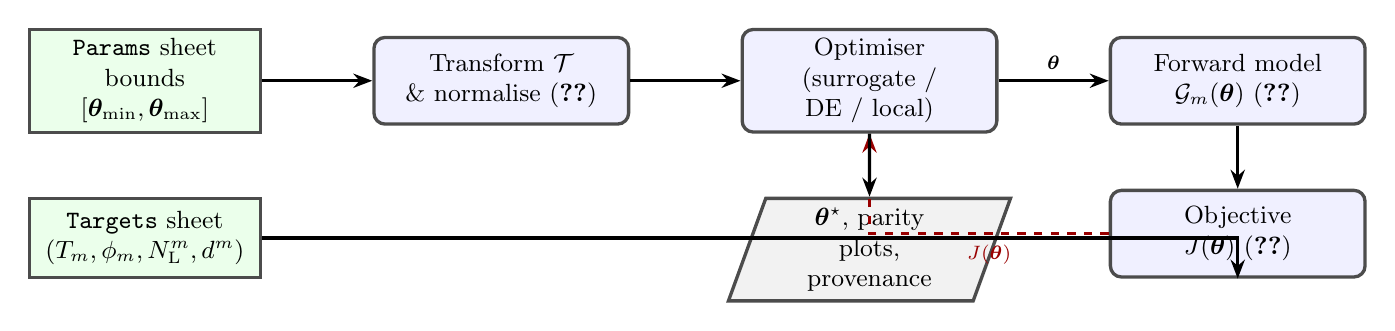
\begin{tikzpicture}[node distance=8mm and 14mm]
  \node[data] (params)  {\texttt{Params} sheet\\bounds $[\param_{\min},\param_{\max}]$};
  \node[data,below=of params] (targets) {\texttt{Targets} sheet\\$(T_m,\dpa_m,\NL^m,d^m)$};
  \node[block,right=of params] (trans) {Transform $\mathcal{T}$\\ \& normalise \eqref{eq:transform}};
  \node[block,right=of trans] (opt) {Optimiser\\(surrogate / DE / local)};
  \node[block,right=of opt] (fwd) {Forward model\\$\mathcal{G}_m(\param)$ \eqref{eq:fwd}};
  \node[block,below=of fwd] (obj) {Objective\\$J(\param)$ \eqref{eq:objective}};
  \node[io,below=of opt] (best) {$\param^{\star}$, parity\\plots, provenance};

  \draw[arr] (params) -- (trans);
  \draw[arr] (trans) -- (opt);
  \draw[arr] (opt) -- node[above,font=\scriptsize]{$\param$} (fwd);
  \draw[arr] (fwd) -- (obj);
  \draw[arr] (targets.east) -| (obj.south);
  \draw[fbk] (obj.west) -| node[below,pos=0.25,font=\scriptsize]{$J(\param)$} (opt.south);
  \draw[arr] (opt) -- (best);
\end{tikzpicture}
\caption{Parameter-identification workflow. The optimiser proposes a parameter
vector, the forward model and observation operator predict the observables, the
objective scores them against the experiments, and the (dashed) feedback drives
the next proposal until convergence or budget exhaustion.}
\label{fig:workflow}
\end{figure}

\begin{figure}[ht]
\centering
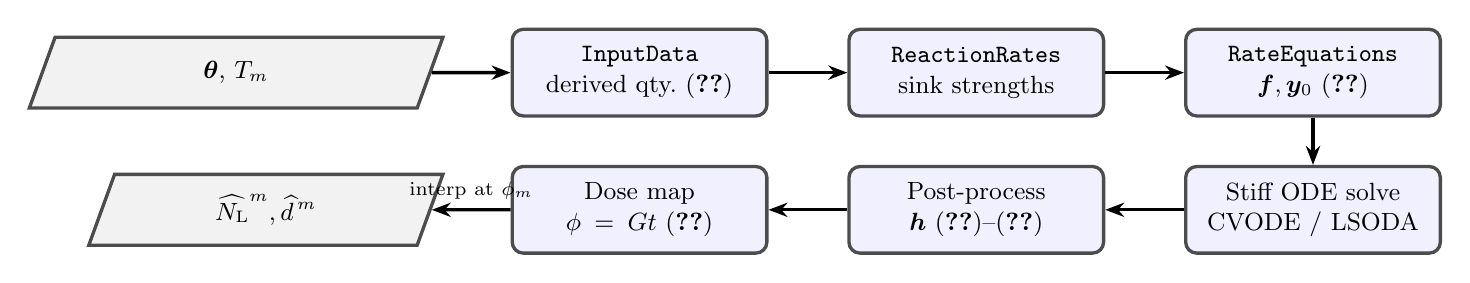
\begin{tikzpicture}[node distance=6mm and 10mm]
  \node[io] (in) {$\param,\,T_m$};
  \node[block,right=of in] (inp)  {\texttt{InputData}\\derived qty.\ \eqref{eq:arrhenius}};
  \node[block,right=of inp] (rr)  {\texttt{ReactionRates}\\sink strengths};
  \node[block,right=of rr] (re)   {\texttt{RateEquations}\\$\bm{f},\bm{y}_0$ \eqref{eq:ode}};
  \node[block,below=of re] (solve){Stiff ODE solve\\CVODE / LSODA};
  \node[block,left=of solve] (post){Post-process\\$\bm{h}$ \eqref{eq:NL}--\eqref{eq:d}};
  \node[block,left=of post] (dose) {Dose map\\$\dpa=Gt$ \eqref{eq:dose}};
  \node[io,left=of dose] (out) {$\widehat{\NL}^{m},\widehat{d}^{\,m}$};

  \draw[arr] (in) -- (inp);
  \draw[arr] (inp) -- (rr);
  \draw[arr] (rr) -- (re);
  \draw[arr] (re) -- (solve);
  \draw[arr] (solve) -- (post);
  \draw[arr] (post) -- (dose);
  \draw[arr] (dose) -- node[above,font=\scriptsize]{interp at $\dpa_m$} (out);
\end{tikzpicture}
\caption{Forward evaluation $\mathcal{G}_m$ for one temperature group. One stiff
integration produces the full time history; the observables at every measured dose
of the group are then obtained by interpolation in $\log_{10}\dpa$.}
\label{fig:forward}
\end{figure}

% =====================================================================
\section{Optimisation algorithms}
% =====================================================================
Three complementary, SciPy-only \citep{Virtanen2020} solvers are provided. They
share the same objective \eqref{eq:objective} and history log, and a final local
polish refines whichever global search is used.

% ---------------------------------------------------------------------
\subsection{Global search: Differential Evolution}
% ---------------------------------------------------------------------
Differential Evolution (DE) \citep{Storn1997} is a robust, derivative-free,
population-based global optimiser. A population
$\{\xv^{(1)},\dots,\xv^{(NP)}\}\subset[\xv_{\min},\xv_{\max}]$ is initialised by a
low-discrepancy (Sobol') sequence. At each generation, every target vector
$\xv^{(s)}$ produces a mutant by combining distinct random members,
\begin{equation}
  \bm{v}^{(s)}=\xv^{(r_1)}+F\big(\xv^{(r_2)}-\xv^{(r_3)}\big),
  \qquad r_1\ne r_2\ne r_3\ne s,
  \label{eq:de-mut}
\end{equation}
with differential weight $F\in(0,2)$. Binomial crossover mixes mutant and target,
\begin{equation}
  u^{(s)}_j=
  \begin{cases}
    v^{(s)}_j, & \text{if } \mathrm{rand}_j\le C_r \ \text{or}\ j=j_{\mathrm{rand}},\\
    x^{(s)}_j, & \text{otherwise,}
  \end{cases}
  \label{eq:de-cross}
\end{equation}
with crossover probability $C_r$, and greedy selection retains the better of trial
and target,
\begin{equation}
  \xv^{(s)}\leftarrow
  \begin{cases}
    \bm{u}^{(s)}, & J(\bm{u}^{(s)})\le J(\xv^{(s)}),\\
    \xv^{(s)},    & \text{otherwise.}
  \end{cases}
  \label{eq:de-sel}
\end{equation}
DE explores the box thoroughly and is insensitive to local minima, at the cost of
many objective evaluations ($\mathcal{O}(NP\times\text{generations})$).

% ---------------------------------------------------------------------
\subsection{Surrogate ``self-learning'' optimisation (RBF)}
% ---------------------------------------------------------------------
When each evaluation is expensive, surrogate-based optimisation (SBO)
\citep{Jones1998,Forrester2009} is far more sample-efficient: a cheap regression
model is \emph{learned} from the evaluated points and minimised to suggest where
to sample next, so the budget is spent where it most reduces the objective. We use
a radial-basis-function (RBF) interpolant \citep{Hardy1971,Wendland2004,Gutmann2001},
the role a trained neural network would play in a learned-surrogate setting.

\paragraph{Initial design.} An $n_0$-point Latin-Hypercube design
\citep{McKay1979} $\{\bm{u}^{(1)},\dots,\bm{u}^{(n_0)}\}$ (with the nominal point
injected) is evaluated, giving data $\mathcal{D}=\{(\bm{u}^{(k)},y^{(k)})\}$,
$y^{(k)}=J(\mathcal{T}^{-1}(\xv^{(k)}))$. By default $n_0=2p+1$.

\paragraph{Surrogate.} Given $\mathcal{D}$, the RBF model is
\begin{equation}
  s(\bm{u})=\sum_{k=1}^{n}\lambda_k\,\psi\big(\lVert\bm{u}-\bm{u}^{(k)}\rVert\big)
  +q(\bm{u}),
  \qquad
  \psi(r)=r^{2}\log r \ \ (\text{thin-plate spline}),
  \label{eq:rbf}
\end{equation}
where $q$ is a low-order polynomial tail. The coefficients $(\bm{\lambda},q)$ solve
the (regularised) interpolation system
\begin{equation}
  \begin{bmatrix} \bm{\Psi}+\sigma\bm{I} & \bm{P}\\ \bm{P}^{\!\top} & \bm{0}\end{bmatrix}
  \begin{bmatrix}\bm{\lambda}\\ \bm{c}\end{bmatrix}
  =\begin{bmatrix}\bm{y}\\ \bm{0}\end{bmatrix},
  \qquad
  \Psi_{kl}=\psi\big(\lVert\bm{u}^{(k)}-\bm{u}^{(l)}\rVert\big),
  \label{eq:rbf-system}
\end{equation}
with $\bm{P}$ the polynomial basis evaluated at the samples and a small smoothing
$\sigma$ for numerical conditioning. The thin-plate spline is scale-free (no shape
parameter to tune) and minimises a second-derivative bending energy, giving a
smooth response surface.

\paragraph{Infill (acquisition).} Each iteration minimises the cheap surrogate over
the unit cube to obtain a candidate,
\begin{equation}
  \bm{u}_{\mathrm{new}}=\operatorname*{arg\,min}_{\bm{u}\in[0,1]^p} s(\bm{u}),
  \label{eq:infill}
\end{equation}
solved with an inner DE on $s$ (negligible cost). To prevent premature
convergence, with probability $p_e$ (default $0.25$) the candidate is replaced by a
uniformly random point --- an explicit exploration/exploitation balance:
\begin{equation}
  \bm{u}_{\mathrm{new}}\leftarrow
  \begin{cases}
    \text{uniform } [0,1]^p, & \text{with prob. } p_e \ (\text{explore}),\\[2pt]
    \operatorname*{arg\,min}_{\bm u} s(\bm u), & \text{with prob. } 1-p_e \ (\text{exploit}).
  \end{cases}
\end{equation}
The new point is evaluated with the true model, appended to $\mathcal{D}$, and the
surrogate is re-fit --- the ``self-learning'' loop (Figure~\ref{fig:surrogate}).
After $n_{\mathrm{infill}}$ iterations the incumbent best is returned. The total
true-model budget is $n_0+n_{\mathrm{infill}}$, typically an order of magnitude
smaller than DE for comparable accuracy.

\begin{figure}[ht]
\centering
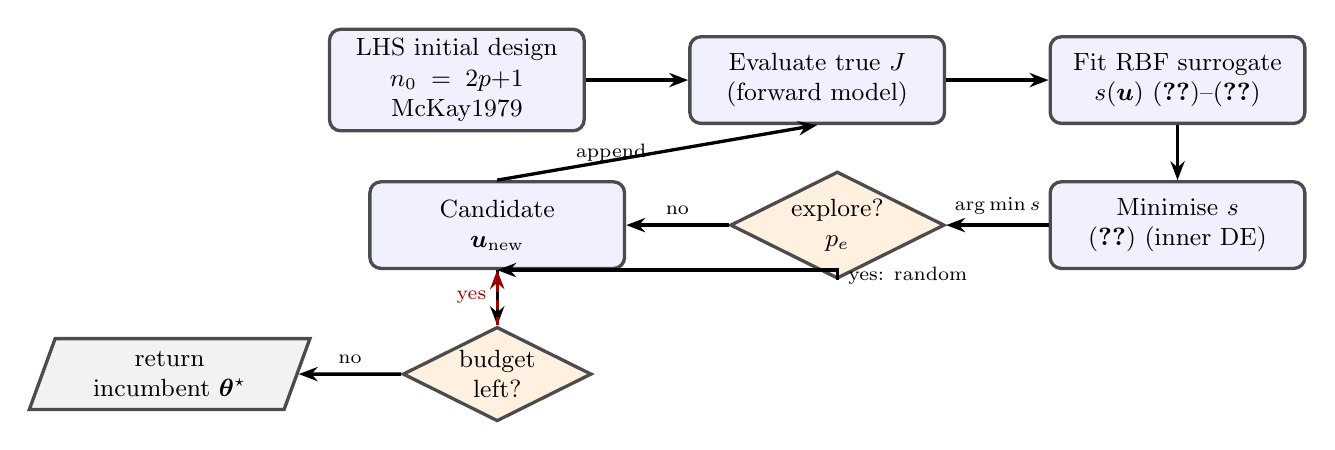
\begin{tikzpicture}[node distance=7mm and 13mm]
  \node[block] (lhs) {LHS initial design\\$n_0=2p{+}1$ \citep{McKay1979}};
  \node[block,right=of lhs] (eval) {Evaluate true $J$\\(forward model)};
  \node[block,right=of eval] (fit) {Fit RBF surrogate\\$s(\bm u)$ \eqref{eq:rbf}--\eqref{eq:rbf-system}};
  \node[block,below=of fit] (min) {Minimise $s$\\ \eqref{eq:infill} (inner DE)};
  \node[decision,left=of min] (expl) {explore?\\$p_e$};
  \node[block,left=of expl] (cand) {Candidate\\$\bm u_{\mathrm{new}}$};
  \node[decision,below=of cand] (stop) {budget\\left?};
  \node[io,left=of stop] (out) {return\\incumbent $\param^{\star}$};

  \draw[arr] (lhs) -- (eval);
  \draw[arr] (eval) -- (fit);
  \draw[arr] (fit) -- (min);
  \draw[arr] (min) -- node[above,font=\scriptsize]{$\arg\min s$} (expl);
  \draw[arr] (expl) -- node[above,font=\scriptsize]{no} (cand);
  \draw[arr] (expl.south) |- node[pos=0.25,right,font=\scriptsize]{yes: random} (cand.south);
  \draw[arr] (cand) -- (stop);
  \draw[fbk] (stop.north) -- node[left,font=\scriptsize]{yes} (cand.south);
  \draw[arr] (cand.north) -- node[left,font=\scriptsize]{append} (eval.south);
  \draw[arr] (stop) -- node[above,font=\scriptsize]{no} (out);
\end{tikzpicture}
\caption{The RBF surrogate ``self-learning'' loop. The surrogate is re-trained on
every newly evaluated point and minimised to choose the next sample, balancing
exploitation (surrogate minimum) against exploration (random infill).}
\label{fig:surrogate}
\end{figure}

\paragraph{Neural-network variant.} The RBF in \eqref{eq:rbf} is one choice of
learned surrogate. If \texttt{PyTorch}/\texttt{scikit-learn} are available, it may
be replaced by a multilayer-perceptron or Gaussian-process regressor trained on
$\mathcal{D}$; the acquisition \eqref{eq:infill} (optionally an expected-improvement
criterion \citep{Jones1998}) and the rest of the loop are unchanged. The RBF is
chosen here for its zero external dependencies and robustness in moderate dimension.

% ---------------------------------------------------------------------
\subsection{Local refinement: Nelder--Mead}
% ---------------------------------------------------------------------
The incumbent from the global stage is polished with the derivative-free
Nelder--Mead downhill-simplex method \citep{NelderMead1965}. A simplex of $p+1$
vertices is iteratively updated by reflection, expansion, contraction, and shrink
operations about the centroid $\bar{\xv}$ of its best $p$ vertices,
\begin{align}
  \xv_{r} &= \bar{\xv}+\alpha(\bar{\xv}-\xv_{p+1}) &&\text{(reflection)},\\
  \xv_{e} &= \bar{\xv}+\gamma(\xv_{r}-\bar{\xv})   &&\text{(expansion)},\\
  \xv_{c} &= \bar{\xv}+\beta(\xv_{p+1}-\bar{\xv})  &&\text{(contraction)},
\end{align}
with standard coefficients $\alpha=1$, $\gamma=2$, $\beta=\tfrac12$ (adaptive
variant for higher $p$). Bounds are enforced by the projection in
\eqref{eq:transform}. Nelder--Mead converges quickly in the neighbourhood of a
minimum but is purely local --- hence its use only as a final polish.

% =====================================================================
\section{Algorithm summary}
% =====================================================================
\begin{algorithm}[ht]
\caption{Surrogate-based parameter identification (default path)}
\label{alg:sbo}
\begin{algorithmic}[1]
\Require bounds $[\param_{\min},\param_{\max}]$, experiments $\{(T_m,\dpa_m,\NL^m,d^m)\}$,
         budgets $n_0,n_{\mathrm{infill}}$, weights $w_{\NL},w_d$, explore prob.\ $p_e$
\State build transform $\mathcal{T}$ \eqref{eq:transform}; group experiments by temperature
\State $\mathcal{D}\gets\varnothing$; draw LHS $\{\bm u^{(k)}\}_{k=1}^{n_0}$, inject nominal point
\For{$k=1,\dots,n_0$}
   \State $y^{(k)}\gets J\big(\mathcal{T}^{-1}(\xv^{(k)})\big)$ \Comment{Alg.~\ref{alg:obj}}
   \State $\mathcal{D}\gets\mathcal{D}\cup\{(\bm u^{(k)},y^{(k)})\}$
\EndFor
\For{$t=1,\dots,n_{\mathrm{infill}}$}
   \State fit RBF $s(\cdot)$ on $\mathcal{D}$ \eqref{eq:rbf-system}
   \State $\bm u_{\star}\gets\arg\min_{\bm u\in[0,1]^p} s(\bm u)$ (inner DE)
   \State $\bm u_{\mathrm{new}}\gets$ random point w.p.\ $p_e$, else $\bm u_{\star}$
   \State $y_{\mathrm{new}}\gets J(\mathcal{T}^{-1}(\xv_{\mathrm{new}}))$;\ \ $\mathcal{D}\gets\mathcal{D}\cup\{(\bm u_{\mathrm{new}},y_{\mathrm{new}})\}$
\EndFor
\State $\param^{\star}\gets$ Nelder--Mead polish from incumbent best \citep{NelderMead1965}
\State \Return $\param^{\star}$, parity plots, comparison table, provenance
\end{algorithmic}
\end{algorithm}

\begin{algorithm}[ht]
\caption{Objective evaluation $J(\param)$}
\label{alg:obj}
\begin{algorithmic}[1]
\Require $\param$ (projected into bounds), grouped experiments
\State $\mathcal{R}_{\NL}\gets[\,]$, $\mathcal{R}_{d}\gets[\,]$
\For{each temperature group $(T,\{\dpa_m,\NL^m,d^m\})$}
   \State configure model with $\param,T$; recompute \eqref{eq:arrhenius}, rebuild $\bm f$
   \State integrate \eqref{eq:ode} to $t_{\mathrm{end}}=10^{\lceil\log_{10}(3\dpa_{\max}/G)\rceil}$
   \If{solve failed} \State \Return $J_{\mathrm{pen}}$ \EndIf
   \State form $\widehat{\NL}(\dpa),\widehat d(\dpa)$ via \eqref{eq:NL}--\eqref{eq:d}; interpolate at each $\dpa_m$
   \State append $r^{\NL}_m,\,r^{d}_m$ for available measurements
\EndFor
\State \Return $w_{\NL}\,\overline{(\mathcal R_{\NL})^2}+w_{d}\,\overline{(\mathcal R_{d})^2}$ \eqref{eq:objective}
\end{algorithmic}
\end{algorithm}

% =====================================================================
\section{Computational cost and practical notes}\label{sec:cost}
% =====================================================================
One objective evaluation integrates \eqref{eq:ode} once per distinct temperature
($\sim\!10$ groups for the present database), at $\sim\!\SI{0.7}{\second}$ each,
i.e.\ $\sim\!\SI{7}{\second}$ per call. The default surrogate budget
($n_0=2p+1$, $n_{\mathrm{infill}}=40$) is a few hundred solves (\(\sim\)10--20 min).
Useful guidance:
\begin{itemize}\setlength\itemsep{1pt}
  \item \textbf{Grouping by temperature} amortises the dominant cost; doses within a
        group are free (interpolation).
  \item \textbf{Log/relative metrics} in \eqref{eq:objective} prevent the few
        high-density points from dominating the fit.
  \item \textbf{Parameters pinned at a bound} in the result table signal either an
        active physical constraint or a too-narrow range --- widen the bound in
        \texttt{Params} and re-run.
  \item \textbf{Reproducibility:} every run writes \texttt{optimal\_parameters.csv},
        \texttt{model\_vs\_experiment.csv}, the parity figure, and a
        \texttt{fit\_provenance.md} to a timestamped \texttt{output/fit\_*} directory.
  \item \textbf{Identifiability:} with $p$ comparable to the number of independent
        measurements, several parameters may be only weakly constrained; a local
        sensitivity/Hessian analysis or Bayesian (MCMC) posterior
        \citep{Tarantola2005} can quantify this and is a natural extension.
\end{itemize}

% =====================================================================
\section{Correspondence to the implementation}
% =====================================================================
The method is implemented as a single self-contained cell in
\texttt{ZrMicro/code/ZrMicro.ipynb}. Table~\ref{tab:map} maps the formulation to
the code.
\begin{table}[ht]
\centering
\small
\begin{tabular}{@{}ll@{}}
\toprule
Formulation & Notebook entity \\
\midrule
$[\param_{\min},\param_{\max}]$, nominal & \texttt{Params} sheet $\to$ \texttt{load\_fit\_tables} \\
$(T_m,\dpa_m,\NL^m,d^m)$ & \texttt{Targets} sheet $\to$ \texttt{TARGETS}, \texttt{TEMP\_GROUPS} \\
transform $\mathcal{T}$ \eqref{eq:transform} & \texttt{LOG\_MASK}, \texttt{\_to\_t}, \texttt{\_from\_t} \\
forward map $\mathcal{G}_m$ \eqref{eq:fwd} & \texttt{predict()} \\
observation operator \eqref{eq:NL}--\eqref{eq:d} & \texttt{predict()} (\texttt{N\_L}, \texttt{d\_mean}) \\
objective $J$ \eqref{eq:objective} & \texttt{objective()} \\
DE / surrogate / local & \texttt{run\_diff\_evol}, \texttt{run\_surrogate}, \texttt{run\_local} \\
outputs & \texttt{output/fit\_<timestamp>\_<git>/} \\
\bottomrule
\end{tabular}
\caption{Mapping between the mathematical formulation and the notebook code.}
\label{tab:map}
\end{table}

% =====================================================================
\begin{thebibliography}{99}
\bibitem[Forrester \& Keane(2009)]{Forrester2009}
A.~I.~J. Forrester and A.~J. Keane,
\emph{Recent advances in surrogate-based optimization},
Progress in Aerospace Sciences \textbf{45} (2009) 50--79.

\bibitem[Gutmann(2001)]{Gutmann2001}
H.-M. Gutmann,
\emph{A radial basis function method for global optimization},
Journal of Global Optimization \textbf{19} (2001) 201--227.

\bibitem[Hardy(1971)]{Hardy1971}
R.~L. Hardy,
\emph{Multiquadric equations of topography and other irregular surfaces},
Journal of Geophysical Research \textbf{76} (1971) 1905--1915.

\bibitem[Jones et al.(1998)]{Jones1998}
D.~R. Jones, M. Schonlau and W.~J. Welch,
\emph{Efficient global optimization of expensive black-box functions},
Journal of Global Optimization \textbf{13} (1998) 455--492.

\bibitem[McKay et al.(1979)]{McKay1979}
M.~D. McKay, R.~J. Beckman and W.~J. Conover,
\emph{A comparison of three methods for selecting values of input variables in the
analysis of output from a computer code},
Technometrics \textbf{21} (1979) 239--245.

\bibitem[Nelder \& Mead(1965)]{NelderMead1965}
J.~A. Nelder and R. Mead,
\emph{A simplex method for function minimization},
The Computer Journal \textbf{7} (1965) 308--313.

\bibitem[Storn \& Price(1997)]{Storn1997}
R. Storn and K. Price,
\emph{Differential evolution -- a simple and efficient heuristic for global
optimization over continuous spaces},
Journal of Global Optimization \textbf{11} (1997) 341--359.

\bibitem[Tarantola(2005)]{Tarantola2005}
A. Tarantola,
\emph{Inverse Problem Theory and Methods for Model Parameter Estimation},
SIAM, Philadelphia, 2005.

\bibitem[Virtanen et al.(2020)]{Virtanen2020}
P. Virtanen et al.,
\emph{SciPy 1.0: fundamental algorithms for scientific computing in Python},
Nature Methods \textbf{17} (2020) 261--272.

\bibitem[Wendland(2004)]{Wendland2004}
H. Wendland,
\emph{Scattered Data Approximation},
Cambridge University Press, 2004.

\bibitem[Christien \& Barbu(2009)]{Christien2009}
F. Christien and A. Barbu,
\emph{Cluster Dynamics modelling of irradiation growth of zirconium single crystals},
Journal of Nuclear Materials \textbf{393} (2009) 153--161.

\bibitem[Was(2017)]{Was2017}
G.~S. Was,
\emph{Fundamentals of Radiation Materials Science: Metals and Alloys},
2nd ed., Springer, 2017.

\bibitem[Jostons et al.(1977)]{Jostons1977}
A. Jostons, P.~M. Kelly and R.~G. Blake,
\emph{The nature of dislocation loops in neutron irradiated zirconium},
Journal of Nuclear Materials \textbf{66} (1977) 236--256.

\bibitem[Northwood(1977)]{Northwood1977}
D.~O. Northwood,
\emph{Irradiation damage in zirconium and its alloys},
Atomic Energy Review \textbf{15} (1977) 547--610.
\end{thebibliography}

\end{document}
